\chapter*{Introduction}
\addcontentsline{toc}{chapter}{Introduction}

% In the recent years, many researchers have been interested by the task of computer vision. 
% 	"task of computer vision" mi pripada zvlastni; task je jeden konkretni ukol, computer vision je cely velky obor, coz moc nejde dohromady; navic asi precijen zacneme trochu konkretneji
The task of reconstructing 3D information from multiple 2D photos of a real-world scene has attracted a lot of research in the last two decades and in the recent years in particular.
% 	tim padem muzeme tohle vyskrtnout 
% Particularly the problem of 3D reconstruction is being investigated a lot. 
% 	Kazdopadne pokracujme... 
% At this moment there is a great number of algorithms to solve problems in this area. 
A great number of algorithms have been proposed to solve problems in this area and several main approaches have emerged. 
% Most of these approaches depend on the kind of input that is available 
% (a set of pictures -- determining is also how many pictures are taken, a video stream, etc.) 
% and also on the output that we expect.
The applicability of these approaches depends mainly on what kind of input we intend to feed the algorithm 
(an unorganized set of photos, a video stream, a pair of stereoscopic images, etc.) 
and also on what type of output we expect the algorithm to produce (polygonal model, a disparity map). 
As a result of this progress, various real-world applications for these algorithms have appeared -- 
e.g., several camera trackers or products like Microsoft PhotoSynth \cite{snavely2008}.

Simultaneously, both the general availability and the computational power of smartphones have improved significantly.
Mobile phones that employ the Linux-based Android software platform are currently very popular. 
The Android market share increased to almost 69\% in the year 2012 \cite{marketshare} (Figure \ref{fig:market_share}). 
A built–in camera, a relatively fast CPU and various sensors such as the accelerometer are very common in such mobile phones, making it possible to develop a wider range of applications.

\begin{figure}[h]
  \centering{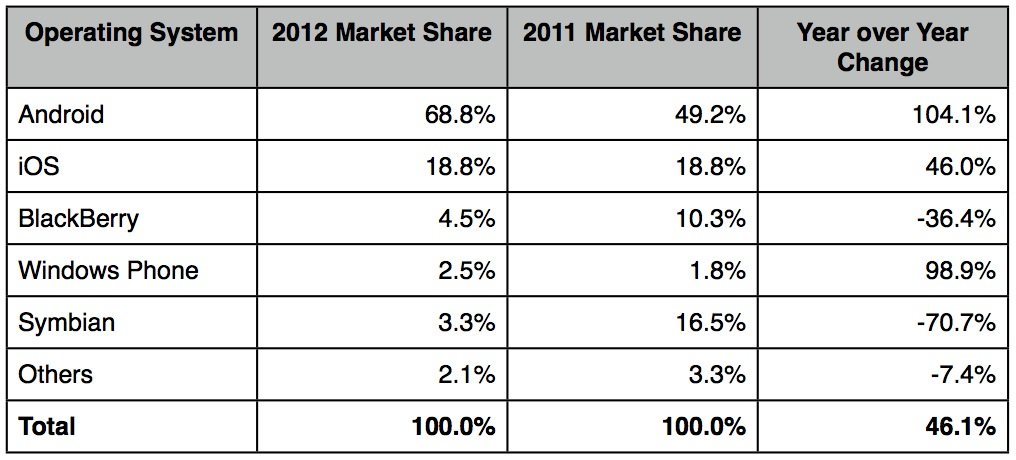
\includegraphics[width=120mm]{img/market_android_table.jpg}}
  \caption{Top five smartphone operating systems and their market share in 2011 and 2012.}
  \label{fig:market_share}
\end{figure}

The goal of this work is to explore the ways of connecting these two phenomena. 
Our aim is to create an Android application that takes a pair of photos using the phone's internal camera, applies a series of \cv\ algorithms to reconstruct the depth information, and visualizes the result using 3D graphics. % XXX
Due to the inherent ambiguity of the problem, it is inevitable that our approach will be limited to particular types of scenes, for example sets of photos of highly textured surfaces. 
% TODO Tuhle vetu zatim vynechavam, protoze je moc odvazna... 
One of our main goals is to investigate how well the solving of such a computation-intesive problem can be done within the limits of a Java-based environment running on a mobile phone or a tablet computer.

\section*{Outline of the thesis}

The first part of this work analyzes the problem, describes currently available software packages solving related tasks, and gives an overview of some of the programming libraries employed in this work (Chapter \ref{chap:overview}). 
There, we also discuss the basic properties of the user supplied input of our reconstruction algorithm. 
These are of great importance since they motivate the subsequent choices we make in the implementation part of the work.
In Chapter \ref{chap:notions}, we introduce the mathematical concepts fundamental to the area of computer vision. 
This part also fixes the notation used in the remaining parts of the thesis. 
In Chapter \ref{chap:algorithms}, we describe several algorithms from the literature that have been successfully applied in software performing automatic 3D reconstruction. 
Then, we elaborate on the basics of Android development (Chapter \ref{chap:android}).
The following section is devoted to the implementation of our application.
We consider the properties of the expected input and choose appropriate algorithms (and their parameters) from which to build our software solution. 
We also discuss and justify our choices. 
Finally, we evaluate and benchmark the resulting application in Chapter \ref{chap:eval}.

